\documentclass[dvipdfmx,11pt,notheorems]{beamer}
%%%% 和文用 %%%%%
\usepackage{bxdpx-beamer}
\usepackage{pxjahyper}
\usepackage{minijs}%和文用
\usepackage{listings,jlisting} % プログラムの表示用
\usepackage{type1cm}
\renewcommand{\kanjifamilydefault}{\gtdefault}%和文用

%%%% tikz 用 %%%%%
\usepackage[latin1]{inputenc}
\usepackage{tikz}
\usetikzlibrary{intersections}
\usetikzlibrary{shapes,arrows}

%%%% スライドの見た目 %%%%%
\usetheme{Boadilla}
\usecolortheme{seahorse}
\usefonttheme{professionalfonts}
\setbeamertemplate{frametitle}[default][center]
\setbeamertemplate{navigation symbols}{}
\setbeamercovered{transparent}%好みに応じてどうぞ)
\setbeamertemplate{footline}[page number]
\setbeamerfont{footline}{size=\normalsize,series=\bfseries}
\setbeamercolor{footline}{fg=black,bg=black}

\setbeamercolor{white-cyan1}
{fg=white,bg=cyan!80!black}
\setbeamercolor{white-cyan2}
{fg=white,bg=cyan!60!black}

%フラットデザイン化
\setbeamertemplate{blocks}[rounded] % Blockの影を消す
%Beamer色設定
\definecolor{UniBlue}{RGB}{0,150,200}
\definecolor{AlertOrange}{RGB}{255,76,0}
\definecolor{AlmostBlack}{RGB}{38,38,38}
\setbeamercolor{structure}{fg=UniBlue} % 見出しカラー
\setbeamercolor{block title}{fg=UniBlue!50!black} % ブロック部分タイトルカラー
%%%%

%%%% 定義環境 %%%%%
\usepackage{amsmath,amssymb}
\usepackage{amsthm}
\usepackage{bm}
\theoremstyle{definition}
\newtheorem{theorem}{定理}
\newtheorem{definition}{定義}
\newtheorem{proposition}{命題}
\newtheorem{lemma}{補題}
\newtheorem{corollary}{系}
\newtheorem{conjecture}{予想}
\newtheorem*{remark}{Remark}
\renewcommand{\proofname}{}
%%%%%%%%%

%%%%% フォント基本設定 %%%%%
% \usepackage[T1]{fontenc}%8bit フォント
% \usepackage{textcomp}%欧文フォントの追加
% \usepackage[utf8]{inputenc}%文字コードをUTF-8
% \usepackage{otf}%otfパッケージ
% \usepackage{lxfonts}%数式・英文ローマン体を Lxfont にする
% \usepackage{bm}%数式太字
%%%%%%%%%%

%%%%% 複数人の著者を揃える %%%%%
%% http://tex.stackexchange.com/questions/
%%   166531/how-to-change-author-alignment-in-beamer
\makeatletter
\long\def\beamer@author[#1]#2{%
  \def\insertauthor{\def\inst{\beamer@insttitle}\def\and{\beamer@andtitle}%
  \begin{tabular}{rl}#2\end{tabular}}%
  \def\beamer@shortauthor{#1}%
  \ifbeamer@autopdfinfo%
    \def\beamer@andstripped{}%
    \beamer@stripands#1 \and\relax
    {\let\inst=\@gobble\let\thanks=\@gobble\def\and{, }\hypersetup{pdfauthor={\beamer@andstripped}}}
  \fi%
}
\makeatother
%%%%%%%%%%

%%%%% プログラムに色をつける
\usepackage{color}

\definecolor{codegreen}{rgb}{0,0.6,0}
\definecolor{codegray}{rgb}{0.5,0.5,0.5}
\definecolor{codepurple}{rgb}{0.58,0,0.82}
\definecolor{backcolour}{rgb}{0.95,0.95,0.92}

\lstdefinestyle{mystyle}{
    backgroundcolor=\color{backcolour},
    commentstyle=\color{codegreen},
    keywordstyle=\color{magenta},
    numberstyle=\tiny\color{codegray},
    stringstyle=\color{codepurple},
    basicstyle=\footnotesize,
    breakatwhitespace=false,
    breaklines=true,
    captionpos=b,
    keepspaces=true,
    numbers=left,
    numbersep=5pt,
    showspaces=false,
    showstringspaces=false,
    showtabs=false,
    tabsize=2
}

\lstset{style=mystyle}

%%%%
\title[略タイトル]{第6回 知能システム学特論レポート}%[略タイトル]{タイトル}
\author[NishidaLab]{
15344203 & 有田 裕太 \\
15344206 & 緒形 裕太 \\
15344209 & 株丹 亮 \\
12104125 & 宮本 和 }%[略名前]{名前}
\institute[NishidaLab]{西田研究室,計算力学研究室}%[略所属]{所属}
\date{2015年\ 7月\ 6日}%日付

\begin{document}

%%%% 1 %%%%
\begin{frame}[plain]\frametitle{}
\titlepage %表紙
\end{frame}

% \begin{frame}\frametitle{Contents}
% \tableofcontents %目次
% \end{frame}

%%%% 進捗状況 %%%%
\begin{frame}\frametitle{進捗状況}

\begin{block}{理論研究の進捗}
畳込みニューラルネットワークの理論について
\end{block}

\vspace{1cm}
\begin{exampleblock}{プログラミングの進捗}
プログラム実行環境の見直し\\
データセット作成
\end{exampleblock}
\end{frame}


%%%% 畳み込みの定義 %%%%
\begin{frame}[fragile]\frametitle{畳み込みの定義}
\begin{itemize}
\item 濃淡地を各画素に格納したグレースケールの画像を考える.
\item 画像サイズを$W\times W$画素,画素をインデックス$(i,j)(i = 0,\cdots,W-1, j = 0,\cdots,W-1)$画素値を$x_{ij}$,\\
フィルタサイズを$H\times H$画素,画素をインデックス$(p,q)(p=0,\cdots,H-1, q=0,\cdots,H-1)$,画素値を$h_{pq}$とすると,
\begin{equation}
  u_{ij} = \sum_{p=0}^{H-1} \sum_{q=0}^{H-1} x_{i+p,j+q} h_{pq}
\end{equation}
\item この計算はフィルタが表す特徴的な濃淡構造を,画像から抽出する「特徴抽出」の働きがある.
\end{itemize}
\end{frame}

%%%% 畳み込みの働き %%%%
\begin{frame}[fragile]\frametitle{畳み込みの働き}

\begin{figure}[t]
 \centering
 \includegraphics[scale=0.3]{fig/eps/convlena.eps}
  \caption{画像の畳み込みの例}
  \label{fig:画像の畳み込みの例}
\end{figure}
\begin{itemize}
 \item 入力画像:227×227
 \item フィルタ:11×11
 \item 出力画像:55×55
 \item ストライド:4
\end{itemize}

\end{frame}


%%%% パディング 1 %%%%
\begin{frame}[fragile]\frametitle{パディング}
\begin{itemize}
\item 畳込みは画像にフィルタを重なり合う画素どおしの積を求めて,フィルタ全体の和を求める.
\item 画像内にフィルタ全体が収まる範囲内でフィルタを動かすと,畳込み処理を行った後の画像サイズは入力画像は小さくなる.
\end{itemize}

\begin{figure}[b]
  \begin{center}
    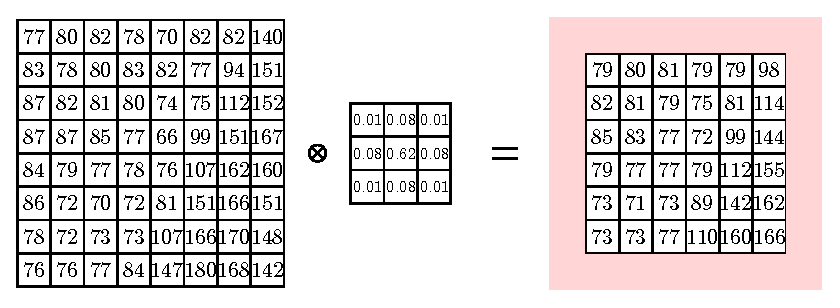
\includegraphics[clip,width=9cm]{fig/eps/convolution.eps}
  \end{center}
  \caption{$8\times 8$の入力画像を畳込み処理した場合の出力画像のサイズ縮小の様子}
  \label{fig:88の入力画像を畳込み処理した場合の出力画像のサイズ縮小の様子}
\end{figure}

\end{frame}

%%%% パディング 2 %%%%
\begin{frame}[fragile]\frametitle{パディング}
\begin{block}{このときの画像サイズは}
\begin{equation}
  \left(W-2\left\lfloor \frac{H}{2}\right\rfloor\right)\times \left(W-2\left\lfloor \frac{H}{2}\right\rfloor\right)
\end{equation}
\end{block}
\begin{itemize}
\item 一方で畳込みの結果が入力画像と同サイズに出力する場合,入力画像の外側に幅$\lfloor H/2\rfloor$の余剰を設け,出力画像が元の入力画像と同サイズになるようにする.
\item 余分に設けた部分の画素値を0とする方法をゼロパディング(zero-padding)と呼ぶ.
\end{itemize}

\begin{figure}[t]
  \begin{center}
    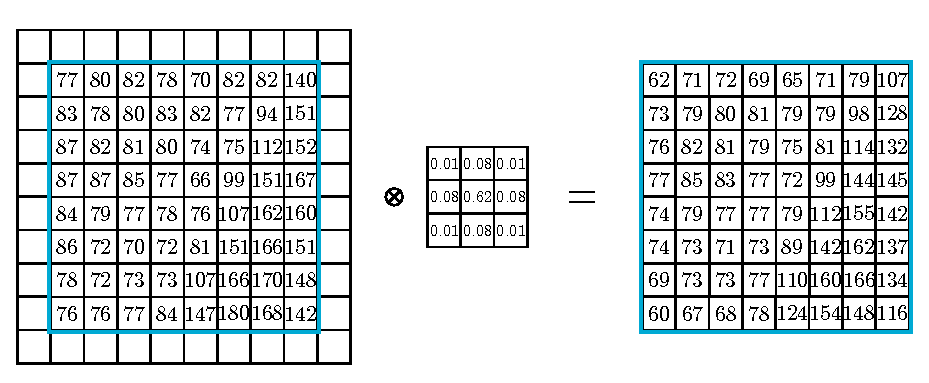
\includegraphics[clip,width=9cm]{fig/eps/zero_padding.eps}
  \end{center}
  % \caption{$8\times 8$の入力画像にゼロパディングを施した場合}
  % \label{fig:88の入力画像にゼロパディングを施した場合}
\end{figure}
\end{frame}

%%%% ストライド 1 %%%%
\begin{frame}[fragile]\frametitle{ストライド}
\begin{block}{ストライド}
フィルタの適用位置を1画素ずつではなく,数画素ずつずらして計算する.このずらす間隔をストライド(stride)という.
\end{block}
ストライドを$s$とするとき,出力画像の画素値は
\begin{eqnarray}
 u_{ij} = \sum^{H-1}_{p=0}\sum^{H-1}_{q=0} x_{si+p,sj+q}h_{pq}
\end{eqnarray}
サイズは
\begin{eqnarray}
 \left(\left[\left(W-1\right)/s\right]+1\right)\times \left(\left[\left(W-1\right)/s\right]+1\right)
\end{eqnarray}
\begin{itemize}
 \item 畳み込み層の出力側のユニット数が大きくなりすぎるのを防ぐために,2以上のストライドが使われることがある
 \item ストライドを大きくすることは画像特徴を取りこぼすことを意味し,性能を悪化させる可能性
\end{itemize}

\end{frame}

%%%% GPUを用いた学習実行時の演算処理高速化 %%%%
\begin{frame}\frametitle{GPUを用いた学習実行時の演算処理高速化}
\begin{itemize}
\item 学習データがあまり多くない場合でも学習を行うことができるファインチューニングを試験的に行った
\item ファインチューニングは大規模なデータセットで学習済みの状態から目的とする別のデータセットへ学習し直す方法
\item CPUのみの演算だと時間がかかりすぎる
\end{itemize}

そこで...
\begin{block}{GPUによる並列計算}
\begin{itemize}
\item caffeがサポートしているNVIDIAの{\color{orange} CUDA}を使う(導入済み)
\item Deep Learning用のCUDAライブラリ{\color{orange} cuDNN}を使用する\\(デベロッパー登録申請中)
\end{itemize}
\end{block}

\begin{figure}[tb]
  \begin{center}
    
\includegraphics[clip,width=6cm]{./fig/eps/GPU.eps}
  \end{center}
\end{figure}

\end{frame}

%%%% 今後の課題 %%%%
\begin{frame}\frametitle{今後の課題}

\begin{block}{理論研究}
CNNの詳細な調査\\
プーリングの理論
\end{block}

\vspace{1cm}
\begin{exampleblock}{プログラミング}
データセットの作成
\end{exampleblock}
\end{frame}

% \begin{figure}[t]
%  \begin{minipage}{0.3\hsize}
%   \centering
%   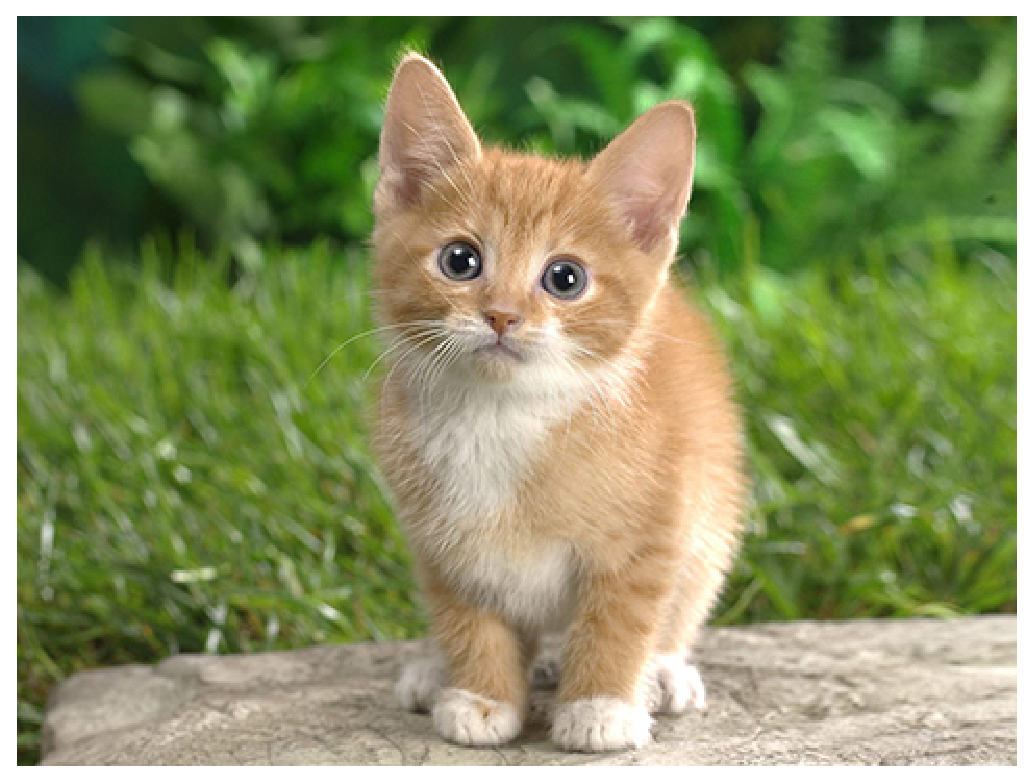
\includegraphics[width=30mm]{./figure/cat.eps}
%   \caption{cat.jpg}
%   \label{sample1}
%  \end{minipage}
%  \begin{minipage}{0.3\hsize}
%   \centering
%   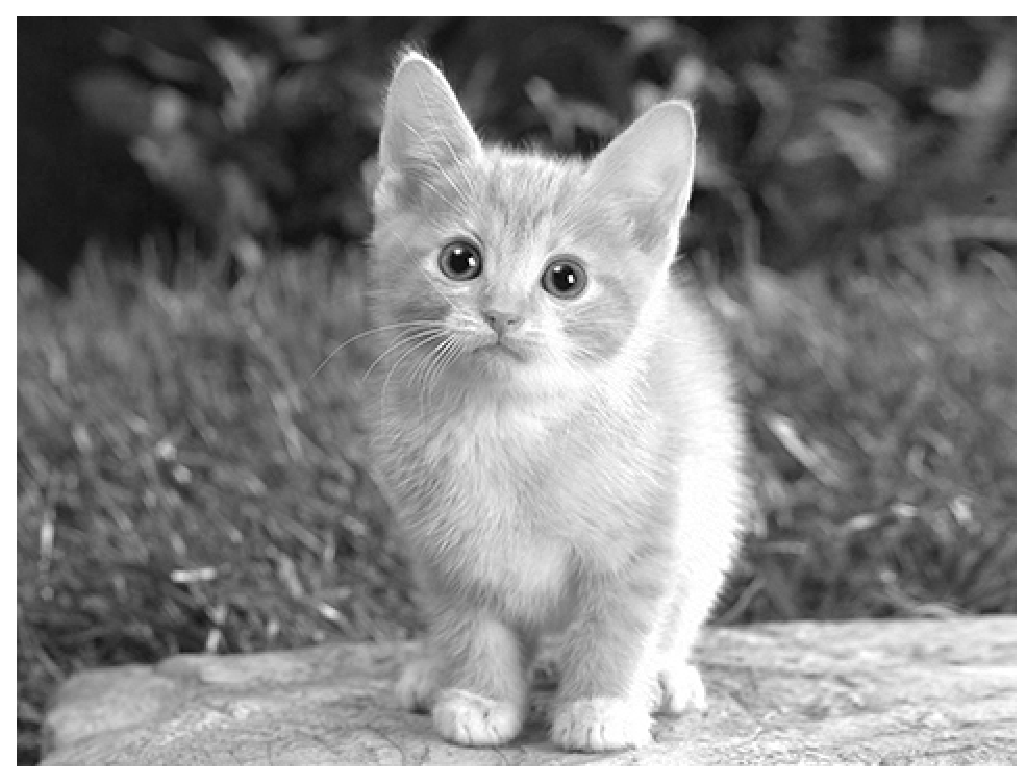
\includegraphics[width=30mm]{./figure/cat_gray.eps}
%   \caption{cat\_gray.jpg}
%   \label{sample2}
%  \end{minipage}
%  \begin{minipage}{0.3\hsize}
%   \centering
%   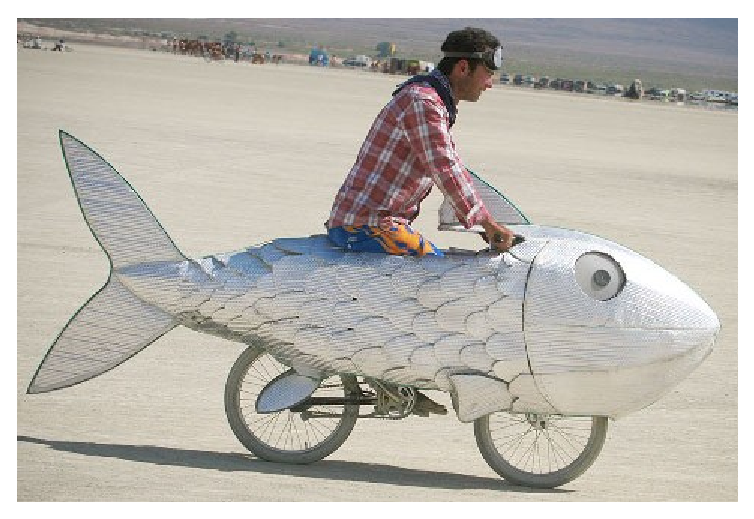
\includegraphics[width=30mm]{./figure/fish-bike.eps}
%   \caption{fish-bike.jpg}
%   \label{sample3}
%  \end{minipage}
% \end{figure}
% \begin{exampleblock}{実行環境}
% \begin{itemize}
%  \item Ubuntu 14.04 LTS
%  \item Intel core i5-4440 3.10GHz$\times$4
%  \item RAM 16GB
% \end{itemize}
% \end{exampleblock}
% \end{frame}


% \section{具体例}

% \begin{frame}\frametitle{定理環境の例}
% \begin{theorem}[Fermat]
% $a^{p-1} \equiv 1 \pmod{p}$
% \end{theorem}
% \pause
% \begin{theorem}[Wilson]
% \begin{equation}
% (p-1)! \equiv 1 \pmod{p}
% \end{equation}
% \end{theorem}
% \end{frame}

% \begin{frame}<1-2>\frametitle{オーバーレイ}
% \onslide*<1>{
% \Large{これは1枚目です}
% }
% \onslide*<2>{
% これは2枚目です
% \begin{theorem}[Euclid]
% There is no largest prime number.
% \end{theorem}
% }
% \end{frame}

% \begin{frame}\frametitle{色もつけれるよ}
%   {\color{red} red}(\alert{alert}),
%   {\color{blue} blue}(\structure{structure}),
%   {\color{green} green},
%   {\color{cyan} cyan},
%   {\color{magenta} magenta},
%   {\color{yellow} yellow},
%   {\color{black} black},
%   {\color{darkgray} darkgray},
%   {\color{gray} gray},
%   {\color{lightgray} lightgray},
%   {\color{orange} orange},
%   {\color{violet} violet},
%   {\color{purple} purple},
%   {\color{brown} brown},
% \end{frame}

% \begin{frame}\frametitle{いろんなブロック}
% \begin{block}{ブロック}
% これは普通のブロックです
% \end{block}

% \begin{alertblock}{警告ブロック}
% 警告!これは警告ブロックだ!
% \end{alertblock}

% \begin{exampleblock}{例ブロック}
% 例えば、こんなブロックです。
% \end{exampleblock}
% \end{frame}

% \begin{frame}<1-2>\frametitle{画像も貼れるよ}
% \onslide*<1>{
% このように画像を貼れるよ
% %\begin{figure}[htb]
% %\centering
% %\includegraphics[width=12cm,clip]{dummygraph.pdf}
% %\caption{$f(x)=e^{-\frac{x}{10}}\sin(x)$}
% %\end{figure}%
% }
% \onslide*<2>{
% 画像や表は各自用意してね
% %\begin{figure}[htb]
% %\centering
% %\includegraphics[width=8cm,clip]{sym4.pdf}
% %\caption{Cayley graph of $\mathfrak{S}_{4}$}
% %\end{figure}%
% }
% \end{frame}

% \begin{frame}\frametitle{まとめ}
% \LARGE{大事なのは中身です!}
% \end{frame}

% \begin{frame}\frametitle{}
% {\Large ありがとうございました}
% \end{frame}
% \appendix

\newcounter{finalframe}
\setcounter{finalframe}{\value{framenumber}}

% \begin{frame}[containsverbatim]\frametitle{dvipngの使い方(1)}
% \begin{block}{この様なファイルを用意する}
% \tiny{
% \begin{verbatim*}
% \documentclass[43pt]{jsarticle}
% \usepackage{amsmath}
% \usepackage{lmodern}
% \pagestyle{empty}
% \begin{document}
% \begin{equation*}
% \sum_{k=0}^{\infty} \frac{(2k)!}{2^{2k}(k!)^2} \frac{1}{2k+1}=\frac{\pi}{2}
% \end{equation*}
% \end{document}
% \end{verbatim*}
% }
% \end{block}
% \end{frame}

% \begin{frame}[containsverbatim]\frametitle{dvipngの使い方(2)}
% \begin{block}{使い方(コマンドライン)}
% \scriptsize{
% \begin{verbatim*}
% latex dvipng-sample.tex
% dvipng dvipng-sample.dvi -T tight -bd 1000
% \end{verbatim*}
% }
% \end{block}
% \end{frame}
\setcounter{framenumber}{\value{finalframe}}
\end{document}